\documentclass{beamer}
\usepackage{amsthm}


\usetheme{Madrid}

\title{Genealogía de la lógica y los conjuntos}
\author{Karina García Buendía}
\date{\today}

\begin{document}

\begin{frame}
\titlepage
\end{frame}

\begin{frame}{¿Por qué estudiar lógica y conjuntos}
    \begin{block}{Según Ferreirós}
        \textit {La lógica y los conjuntos se consieran los fundamentos de
        las matemáticas porque\dots}
        \pause
        \begin{enumerate}
            \item expresan razonamientos matemáticos sin interpretación,
            \item definen conceptos,
            \item establece cuándo un argumento es válido, 
            \item entre otras razones.
        \end{enumerate}
        \pause
    \end{block}
     
        Según el filósofo e historiador de las matemáticas José Ferreirós, la lógica moderna se consolidó 
        en estrecha relación con los problemas de la fundamentación de las matemáticas entre 1850 y 1950.
   \end{frame}

    \begin{frame}{¿Qué es la lógica?}
        Estudia las condiciones de validez de los razonamientos en el marco de un Sistema Formal, ya que le interesa:    

        \begin{enumerate}
            \item las inferencias,
            \item las estructuras formales y
            \item las relaciones entre proposiciones
        \end{enumerate}

    \begin{block}{Ejemplo estudiado desde Aristóteles}
         \textit {Si todas las mujeres no son hombres y los hombres son inteligentes, entonces todas
         las mujeres no son inteligentes.} 
    \end{block}
\end{frame}

\begin{frame}{Ejemplo más contemporáneo}
     \begin{block}{Axioma de la autonomía}
        Todo individuo tiene derecho exclusivo y soberano sobre su propio cuerpo.
     \end{block}
     \pause
         \begin{block}{Axioma de la no obligatoriedad}
        El derecho a la vida de un individuo \textit{X} no implica el derecho a utilizar el cuerpo de un
        individuo \textit{Y} para mantenerse con vida sin el consentimiento explícito de \textit{Y}.
     \end{block}
     \pause
     Supongamos que Isaac Herzog despierta una mañana en un hospital y descubres que estás conectado, 
     mediante un sistema circulatorio compartido, a Donald John Trump que sufre una enfermedad renal 
     fatal. Solo el presidente de Israel tienes el tipo de sangre necesario para filtrar la sangre de Trump;
    si se desconecta, Trump morirá. El hospital informa que Herzog debe permanecer conectado durante 9 meses
     para que se recupere.       
\end{frame}

\begin{frame}
    \begin{block}{Deducción}
        \begin{enumerate}
            \item Si Trump es un individuo con derecho a la vida, ese derecho no le otorga el derecho
            sobre la sangre y los riñones de Isaac Herzog.
            \pause
            \item El derecho de la vida de Trump no puede estar por encima del consentimiento explícito
            de no prestar soporte vital.
            \pause
            \item La interrupción del soporte vital hace alución al Axioma de la autonomía.
        \end{enumerate}
    \end{block}

    \begin{block}{Lema del consentimiento}
        El consentimiento no es transferible. Realizar una acción que tiene una alta probabilidad
        de crear una necesidad de soporte vital, no constituye un contrato irrevocable sobre el uso
        del cuerpo propio.
    \end{block}
\end{frame}

\begin{frame}{¿Qué es la teoría de conjuntos?}
    Es la teoría que no define qué es un conjunto pero nos dice qué se puede y no se puede hacer con esto.
    Hay varias versiónes para no caer en paradojas y la más usada en matemáticas es la de Zermelo.
    \vspace{\baselineskip}
    \pause

    La idea principal es que gran parte de las matemáticas puede construirse a partir de conjuntos.
    \vspace{\baselineskip}
    \pause

    La lógica y los conjuntos pueden responder preguntas como las siguientes:
    \begin{enumerate}
        \item ¿qué es una demostración?
        \item ¿qué objetos existen en matemáticas?
    \end{enumerate}
\end{frame}

\begin{frame}{Genealogía de la lógica según Ferreirós}
    Él investiga que la lógica moderna surge de un proceso histórico en dos fases:
    \begin{enumerate}
        \item Expansión de la lógica. Siglo XIX.
        \pause
        \begin{enumerate}
            \item La lógica se amplía para incluir: relaciones, conjuntos y cuantificadores.
        
          \vspace{\baselineskip}
          \pause
        \end{enumerate}
        \item Restricción de la lógica. Siglo XX.
    
          \pause
        \begin{enumerate}
            \item Después de las paradojas de la teoría de conjuntos, los lógicos restringen la lógica al
            sistema que denominaron lógica de primer orden.

            \vspace{\baselineskip}

            Este proceso muestra que la lógica no es una estructura eterna, sino una construcción histórica y social.
        \end{enumerate}
    \end{enumerate}
\end{frame}

\begin{frame}{Antecedentes históricos}
    Aristóteles (384-322 a. C.) es el fundador de la lógica formal. Sus aportaciones son:
    \begin{enumerate}
        \item Teoría de los silogismos
        \item Análisis de inferencias
    \end{enumerate}
    \vspace{\baselineskip}
    \pause

    Chrysippus y la lógica estoica.
    \vspace{\baselineskip}

    \begin{enumerate}
        \item Proposiciones
        \item Conectivos lógicos
    \end{enumerate}
    Ejemplo. Si llueve, entonces el suelo está mojado.
\end{frame}

\begin{frame}{Revolución lógica del siglo XIX}
    En el siglo XIX la lógica cambia radicalmente. Los personajes\dots
    \begin{center}
    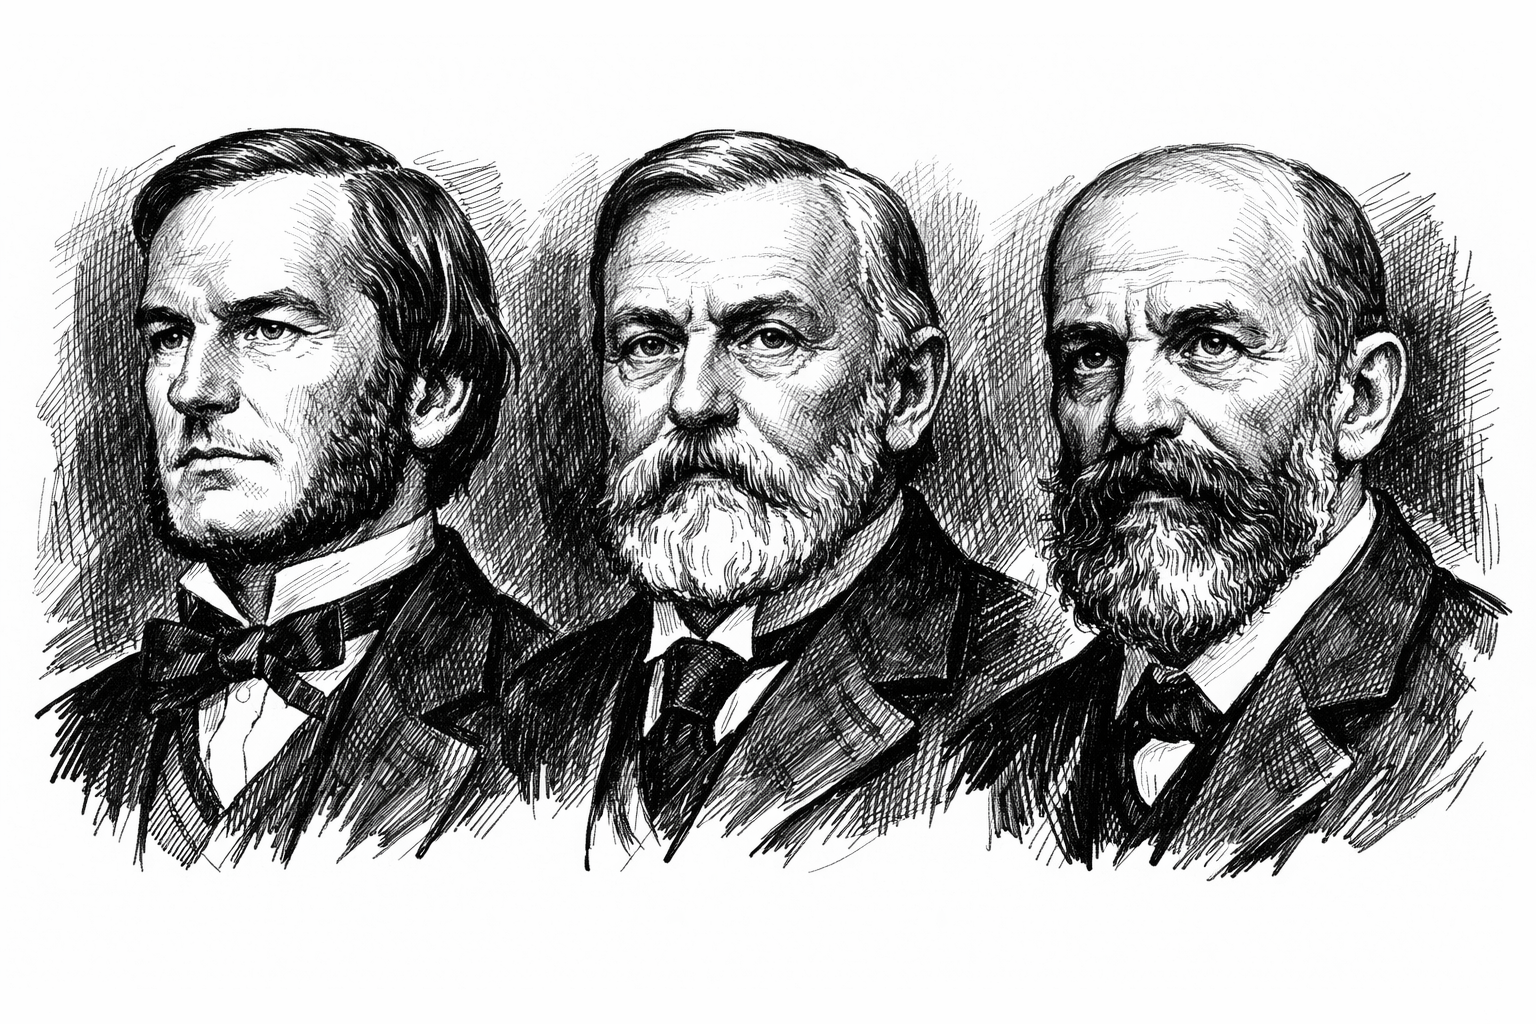
\includegraphics[width=0.7\textwidth]{Peano, Frege y Boole.png}    
    \end{center}
    George Boole, quien introduce el álgebra a la lógica. Gottlob Frege quien crea la lógica moderna 
    e introduce cuantificadores y Giuseppe Peano quien formaliza la aritmética.
\end{frame}

\begin{frame}{Orígenes de la teoría de conjuntos}
    Cantor planteo los diferentes conjuntos infinitos, números transfinito y la jerarquía de los infinitos.
    \begin{center}
    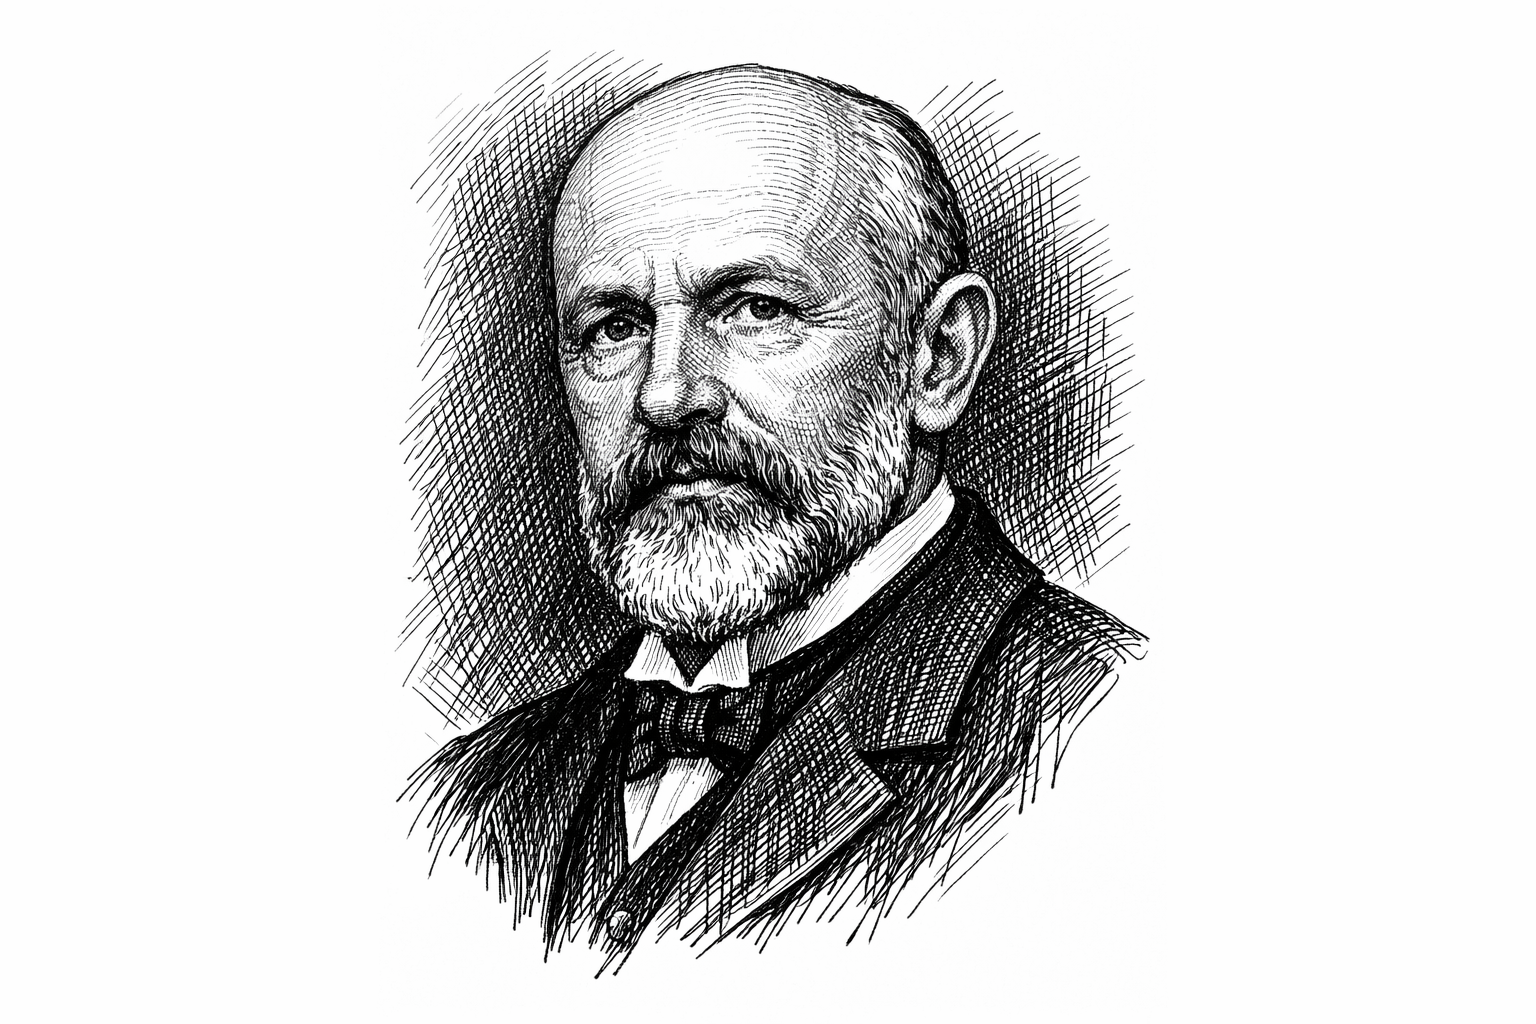
\includegraphics[width=0.7\textwidth]{Cantor.png}
    \end{center}
\end{frame}

\begin{frame}{Crisis de los fundamento}
    Entre 1900 y 1930 se desarrolló la teoría de conjuntos en la que se produjo paradojas.
    \vspace{\baselineskip}
    Como respuesta se plantearon tres programas:
    \begin{enumerate}
        \item Logicismo, representado pro Frege y Russell. \pause Su objetivo era reducir las matemáticas
        a la lógica.
        \item Formalismo, representado por Hilbert. \pause Su objetivo era demostrar que las matemáticas son
        consistentes.
        \item Intuicionismo. L. E. J. Brouwer. \pause Su objetivo es que las matemáticas deben construirse.
    \end{enumerate}
\end{frame}

\begin{frame}{Kurt Gödel}
    Demostró el teorema de incompletitud en 1931. Mostrando que ningún sistiema formal, que pueda expresar y
    desarrollar cierta cantidad mínima de aritmética, puede demostrar su propia consistencia.
    \begin{center}
    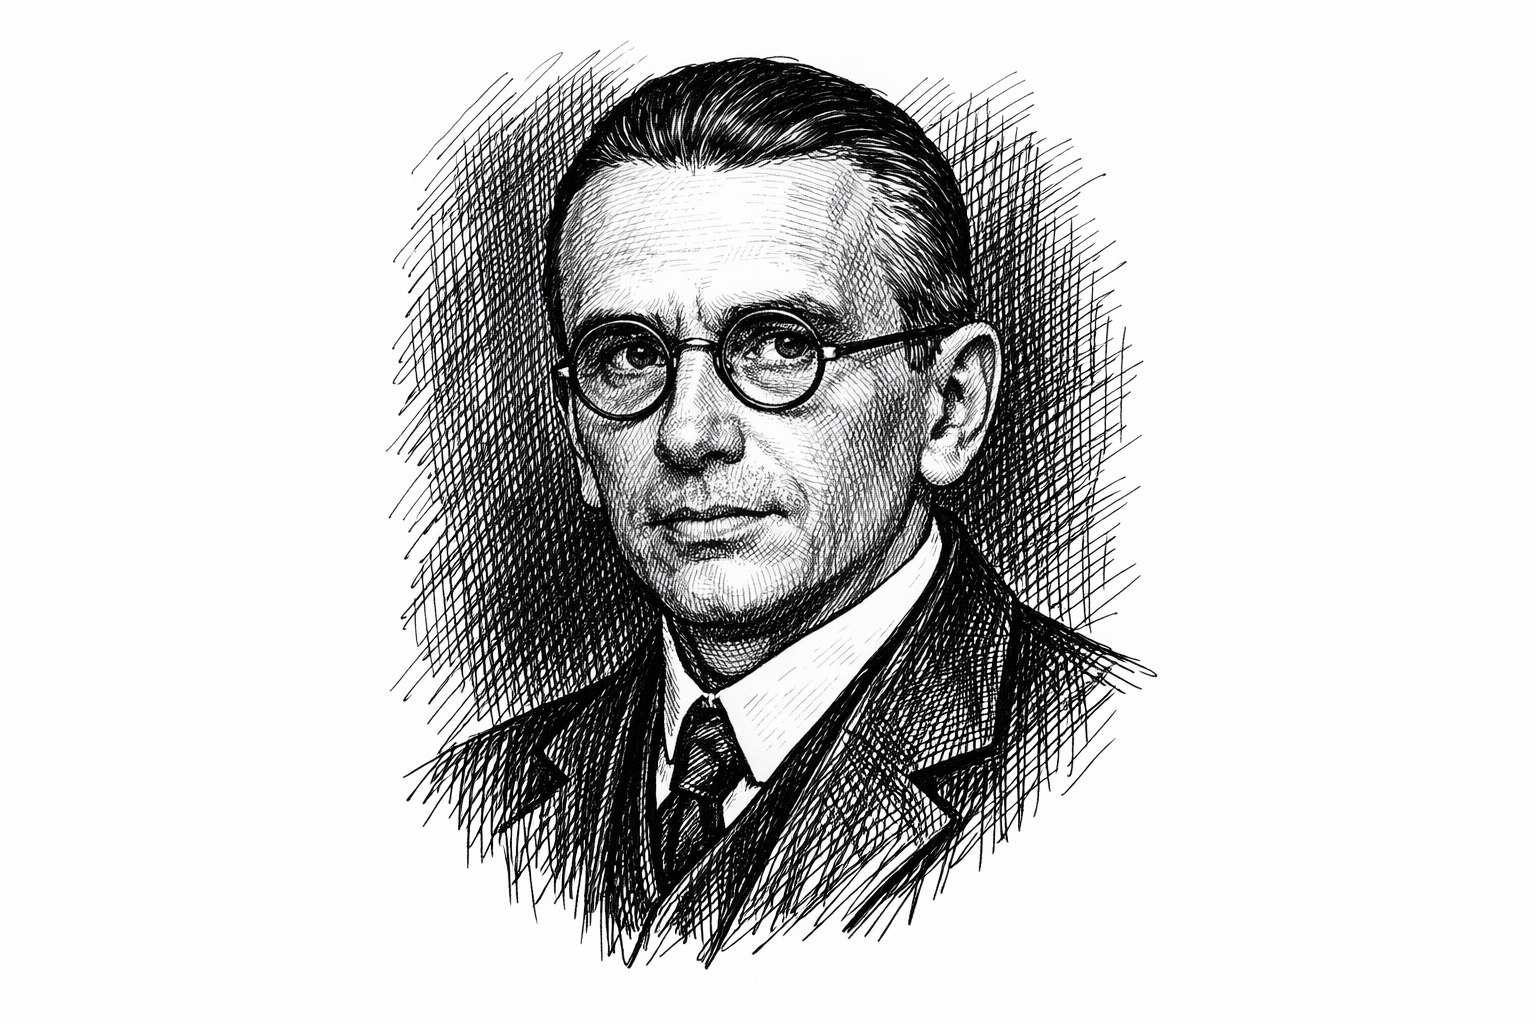
\includegraphics[width=0.7\textwidth]{Godel.png}
    \end{center}
\end{frame}

\begin{frame}{Todo esto tiene otra perspectiva}
    La filósofa de la ciencia Sandra Harding propone la idea de objetividad fuerte, esto se que
    no podemos invisibilizar al contexto social de quién produce conocimiento.
    \pause

    \vspace{0.5cm}
    \begin{center}
        \Large Continuará\dots
    \end{center}
    
\end{frame}

\end{document}
